\chapter{The Evidence Lower Bound (ELBO)}
\label{chap:elbo}

\section{The Problem of Intractable Inference}

The ambition of deep generative modeling is to discover the hidden, low-dimensional factors that give rise to the high-dimensional data we observe in the real world. From images of human faces to the complex waveforms of human speech, we postulate the existence of a latent variable $z \in \mathcal{Z}$ that fundamentally describes an observation $x \in \mathcal{X}$. The generative process is governed by a joint probability distribution $p_\theta(x, z) = p_\theta(x|z)p(z)$, where $p(z)$ is a prior distribution over the latent space and $p_\theta(x|z)$ is the likelihood function parameterized by a powerful function approximator, typically a deep neural network with weights $\theta$.

If we wish to learn the parameters $\theta$ that best explain our dataset $\mathcal{D}$, the principle of maximum likelihood dictates that we should maximize the marginal likelihood, also known as the \textit{evidence}. The evidence is obtained by marginalizing out all possible latent configurations:
\begin{equation}
    p_\theta(x) = \int p_\theta(x|z) p(z) \, dz.
\end{equation}
In all but the simplest linear-Gaussian models, this integral is analytically intractable. The latent space $\mathcal{Z}$ is typically high-dimensional, rendering numerical quadrature impossible. Brute-force Monte Carlo integration is equally hopeless due to the curse of dimensionality; for complex models, the vast majority of sampled $z$ vectors will produce a near-zero likelihood $p_\theta(x|z)$, meaning the variance of naive sampling estimates is astronomically high.

A related, and equally insurmountable, challenge is probabilistic inference. If we observe a datum $x$, what were the specific latent factors $z$ that generated it? Bayes' theorem provides the formal answer via the posterior distribution:
\begin{equation}
    p_\theta(z|x) = \frac{p_\theta(x|z) p(z)}{p_\theta(x)}.
\end{equation}
Because the denominator is the intractable evidence $p_\theta(x)$, evaluating the true posterior $p_\theta(z|x)$ is correspondingly intractable. We are confronted with a chicken-and-egg problem: we need the posterior to understand the internal representations of our data and to properly update our parameters, but we cannot compute the posterior without evaluating the very integral we cannot solve. Without access to the posterior, we cannot apply the Expectation-Maximization (EM) algorithm or any standard likelihood-based optimization technique.

The elegant resolution to this profound mathematical impasse is \textit{variational inference}. Instead of attempting to compute the exact posterior $p_\theta(z|x)$ via brute-force integration, we introduce a new, completely tractable distribution $q_\phi(z|x)$. This distribution—often called the \textit{variational distribution}, \textit{inference model}, or simply the \textit{encoder}—is parameterized by its own set of distinct parameters $\phi$ (such as the weights of a secondary neural network). We then profoundly reframe the problem of Bayesian inference as a problem of pure optimization: we seek to find the parameters $\phi$ that make our tractable $q_\phi(z|x)$ as close as possible to the intractable true posterior $p_\theta(z|x)$.

This shift from integration to optimization is the cornerstone of modern approximate inference. By constructing a lower bound on the log-evidence—the Evidence Lower Bound (ELBO)—we create a surrogate objective function that can be efficiently, jointly optimized with respect to both the generative parameters $\theta$ and the variational parameters $\phi$ using standard stochastic gradient descent. The ELBO not only provides a mathematically rigorous, tractable proxy for maximum likelihood estimation, but it also elegantly bridges the disciplines of information theory, Bayesian statistics, and deep representation learning.

\section{Derivation of the Evidence Lower Bound}

We now formally derive the ELBO. The mathematical machinery relies on the foundational concepts of Kullback-Leibler (KL) divergence and Jensen's inequality. 

\begin{theorem}[The ELBO Decomposition]
\label{thm:elbo_decomp}
Let $p_\theta(x, z)$ be a generative model with latent variables $z$ and observations $x$. Let $q_\phi(z|x)$ be an arbitrary conditional distribution over the latent variables given the observations, with support encompassing that of $p_\theta(z|x)$. The log-marginal likelihood $\log p_\theta(x)$ can be uniquely decomposed as:
\begin{equation}
    \log p_\theta(x) = \mathrm{ELBO}(x; \theta, \phi) + D_{\mathrm{KL}}(q_\phi(z|x) \parallel p_\theta(z|x)),
\end{equation}
where the Evidence Lower Bound (ELBO) is defined as:
\begin{equation}
    \mathrm{ELBO}(x; \theta, \phi) \triangleq \mathbb{E}_{q_\phi(z|x)}\left[ \log \frac{p_\theta(x, z)}{q_\phi(z|x)} \right].
\end{equation}
\end{theorem}

\begin{proof}
By definition of the marginal likelihood, we can write $\log p_\theta(x)$ as the expectation of a constant with respect to the distribution $q_\phi(z|x)$, since $p_\theta(x)$ does not depend on $z$:
\begin{equation}
    \log p_\theta(x) = \mathbb{E}_{q_\phi(z|x)}[ \log p_\theta(x) ].
\end{equation}
Using Bayes' theorem, we can expand the marginal likelihood inside the expectation as $p_\theta(x) = \frac{p_\theta(x, z)}{p_\theta(z|x)}$:
\begin{equation}
    \log p_\theta(x) = \mathbb{E}_{q_\phi(z|x)}\left[ \log \frac{p_\theta(x, z)}{p_\theta(z|x)} \right].
\end{equation}
We then multiply the numerator and denominator inside the logarithm by the variational distribution $q_\phi(z|x)$:
\begin{equation}
    \log p_\theta(x) = \mathbb{E}_{q_\phi(z|x)}\left[ \log \left( \frac{p_\theta(x, z)}{q_\phi(z|x)} \frac{q_\phi(z|x)}{p_\theta(z|x)} \right) \right].
\end{equation}
Using the properties of logarithms, we separate this into two expectations:
\begin{equation}
    \log p_\theta(x) = \mathbb{E}_{q_\phi(z|x)}\left[ \log \frac{p_\theta(x, z)}{q_\phi(z|x)} \right] + \mathbb{E}_{q_\phi(z|x)}\left[ \log \frac{q_\phi(z|x)}{p_\theta(z|x)} \right].
\end{equation}
The first term is precisely the definition of the ELBO. The second term is, by definition, the Kullback-Leibler divergence from the variational distribution to the true posterior. Thus, we arrive at the result:
\begin{equation}
    \log p_\theta(x) = \mathrm{ELBO}(x; \theta, \phi) + D_{\mathrm{KL}}(q_\phi(z|x) \parallel p_\theta(z|x)).
\end{equation}
\end{proof}

\begin{corollary}[The Lower Bound Property]
Because the Kullback-Leibler divergence is non-negative for any two valid probability distributions (a consequence of Gibbs' inequality), i.e., $D_{\mathrm{KL}}(P \parallel Q) \geq 0$, it strictly follows that:
\begin{equation}
    \log p_\theta(x) \geq \mathrm{ELBO}(x; \theta, \phi).
\end{equation}
The bound is tight (holds with exact equality) if and only if $q_\phi(z|x) = p_\theta(z|x)$ almost everywhere, which occurs when the variational distribution perfectly matches the true posterior, implying $D_{\mathrm{KL}}(q_\phi(z|x) \parallel p_\theta(z|x)) = 0$.
\end{corollary}

An alternative, perhaps more direct, derivation of the lower bound property invokes Jensen's inequality applied to the concave logarithm function.

\begin{proof}[Alternative Proof via Jensen's Inequality]
We begin with the definition of the log-marginal likelihood:
\begin{equation}
    \log p_\theta(x) = \log \int p_\theta(x, z) \, dz.
\end{equation}
We multiply and divide the integrand by the variational distribution $q_\phi(z|x)$:
\begin{equation}
    \log p_\theta(x) = \log \int q_\phi(z|x) \frac{p_\theta(x, z)}{q_\phi(z|x)} \, dz = \log \mathbb{E}_{q_\phi(z|x)}\left[ \frac{p_\theta(x, z)}{q_\phi(z|x)} \right].
\end{equation}
Because the logarithm is a strictly concave function, we apply Jensen's inequality ($\log \mathbb{E}[Y] \geq \mathbb{E}[\log Y]$):
\begin{equation}
    \log p_\theta(x) \geq \mathbb{E}_{q_\phi(z|x)}\left[ \log \frac{p_\theta(x, z)}{q_\phi(z|x)} \right] = \mathrm{ELBO}(x; \theta, \phi).
\end{equation}
\end{proof}

This decomposition elegantly illustrates the dual nature of optimizing the ELBO. Because $\log p_\theta(x)$ depends only on $\theta$ and is independent of $\phi$, maximizing the ELBO with respect to $\phi$ strictly minimizes the KL divergence $D_{\mathrm{KL}}(q_\phi(z|x) \parallel p_\theta(z|x))$. In doing so, it forces our approximate posterior to better represent the true posterior. Conversely, maximizing the ELBO with respect to $\theta$ pushes up the lower bound, thereby implicitly maximizing the log-evidence of the data itself.

\begin{figure}[htbp]
\centering
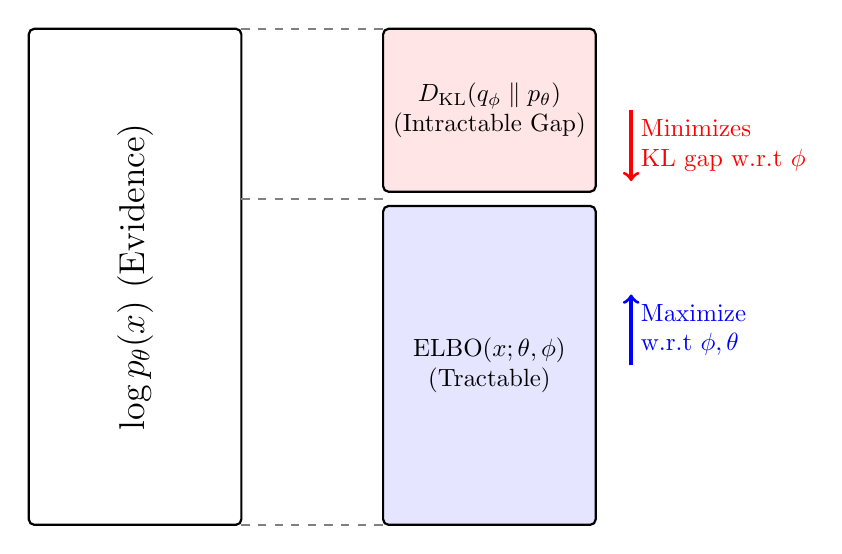
\begin{tikzpicture}[scale=0.9, every node/.style={transform shape}]
    % Total log p(x) block
    \draw[thick, rounded corners=2pt] (0,0) rectangle (3, 7);
    \node[rotate=90, font=\Large] at (1.5, 3.5) {$\log p_\theta(x)$ (Evidence)};
    
    % ELBO block
    \draw[fill=blue!10, thick, rounded corners=2pt] (5,0) rectangle (8, 4.5);
    \node[align=center] at (6.5, 2.25) {$\mathrm{ELBO}(x; \theta, \phi)$ \\ (Tractable)};
    
    % KL block
    \draw[fill=red!10, thick, rounded corners=2pt] (5,4.7) rectangle (8, 7);
    \node[align=center] at (6.5, 5.85) {$D_{\mathrm{KL}}(q_\phi \parallel p_\theta)$ \\ (Intractable Gap)};
    
    % Connections
    \draw[dashed, gray, thick] (3,0) -- (5,0);
    \draw[dashed, gray, thick] (3,7) -- (5,7);
    \draw[dashed, gray, thick] (3,4.6) -- (5,4.6);
    
    % Arrows showing optimization
    \draw[->, very thick, blue] (8.5, 2.25) -- ++(0, 1) node[midway, right, align=left] {Maximize \\ w.r.t $\phi, \theta$};
    \draw[->, very thick, red] (8.5, 5.85) -- ++(0, -1) node[midway, right, align=left] {Minimizes \\ KL gap w.r.t $\phi$};
\end{tikzpicture}
\caption{The Geometry of the Evidence Lower Bound. The log-evidence $\log p_\theta(x)$ is a fixed quantity for a given $\theta$. By maximizing the ELBO with respect to the variational parameters $\phi$, we squeeze the strictly positive KL divergence gap, tightening the bound.}
\label{fig:elbo_geometry}
\end{figure}

\section{Information-Theoretic Interpretation of the ELBO}

The ELBO can be algebraically rearranged into a form that exposes its profound connection to information theory and autoencoding. By expanding the joint distribution $p_\theta(x, z) = p_\theta(x|z)p(z)$, we rewrite the ELBO as:
\begin{align}
    \mathrm{ELBO}(x; \theta, \phi) &= \mathbb{E}_{q_\phi(z|x)}\left[ \log \frac{p_\theta(x|z)p(z)}{q_\phi(z|x)} \right] \nonumber \\
    &= \mathbb{E}_{q_\phi(z|x)}[ \log p_\theta(x|z) ] + \mathbb{E}_{q_\phi(z|x)}\left[ \log \frac{p(z)}{q_\phi(z|x)} \right] \nonumber \\
    &= \mathbb{E}_{q_\phi(z|x)}[ \log p_\theta(x|z) ] - D_{\mathrm{KL}}(q_\phi(z|x) \parallel p(z)).
\end{align}

This formulation reveals the ELBO as a principled trade-off between two distinct information-theoretic forces:
\begin{enumerate}
    \item \textbf{Reconstruction Likelihood:} The term $\mathbb{E}_{q_\phi(z|x)}[ \log p_\theta(x|z) ]$ measures how well the decoder $p_\theta(x|z)$ can reconstruct the data $x$ given latent representations $z$ sampled from the encoder $q_\phi(z|x)$. This acts as a data-fitting or distortion-minimizing term.
    \item \textbf{Complexity Penalty (Regularization):} The term $D_{\mathrm{KL}}(q_\phi(z|x) \parallel p(z))$ quantifies the information cost of encoding the data. It measures how much the variational posterior deviates from the uninformative prior $p(z)$. From an information-theoretic lens, this is the rate of information transmitted from the data to the latent space; penalizing it strictly limits the capacity of the latent channel, thereby compressing the representation.
\end{enumerate}

This tension perfectly mirrors the Information Bottleneck principle discussed earlier in Chapter 8. We are maximizing the mutual information between the latent representation and the observation (by ensuring the latents can decode the observation) while minimizing the information the latents carry about the observation beyond what is strictly necessary (by forcing the posterior to match a naive prior).

\begin{figure}[htbp]
\centering
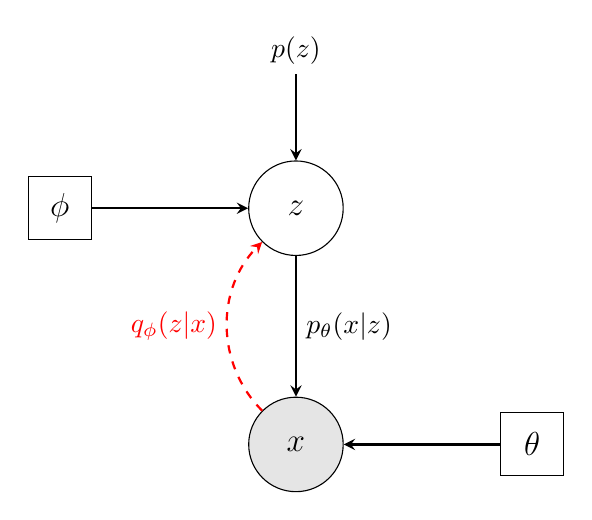
\begin{tikzpicture}[
    obs/.style={circle, draw, fill=gray!20, minimum size=1.2cm, font=\large},
    lat/.style={circle, draw, minimum size=1.2cm, font=\large},
    param/.style={rectangle, draw, minimum size=0.8cm, font=\large},
    arr/.style={-stealth, thick},
    var_arr/.style={-stealth, thick, dashed, red}
]
    % Nodes using absolute coordinates for reliability
    \node[lat] (z) at (0, 3) {$z$};
    \node[obs] (x) at (0, 0) {$x$};
    \node[param] (phi) at (-3, 3) {$\phi$};
    \node[param] (theta) at (3, 0) {$\theta$};
    \node (prior) at (0, 5) {$p(z)$};
    
    % Generative paths
    \draw[arr] (prior) -- (z);
    \draw[arr] (z) -- node[right, pos=0.5] {$p_\theta(x|z)$} (x);
    \draw[arr] (theta) -- (x);
    
    % Variational paths
    \draw[var_arr] (x) to[bend left=45] node[left, pos=0.5] {$q_\phi(z|x)$} (z);
    \draw[arr] (phi) -- (z);
\end{tikzpicture}
\caption{Graphical model depicting the generative process and the variational inference model. Solid black lines represent the generative model parameters $\theta$ dictating the mapping from latents to observations. The dashed red line represents the parameterized encoder $\phi$ actively inferring latents from data.}
\label{fig:elbo_graphical}
\end{figure}

\section{A Tractable Numerical Example: Linear Gaussian Model}

To concretely demonstrate the internal mechanics of the ELBO, we turn to a scenario where the integrals \textit{are} entirely tractable, allowing us to explicitly calculate both the true posterior and the KL divergence gap. Let the true generative model be a scalar linear Gaussian:
\begin{align}
    \text{Prior:} \quad & p(z) = \mathcal{N}(z; 0, 1) \\
    \text{Likelihood:} \quad & p_\theta(x|z) = \mathcal{N}(x; z, \sigma^2).
\end{align}
Because both the prior and likelihood are Gaussian and their relationship is linear, the true posterior and the marginal likelihood are analytically available in closed form. By completing the square on the exponent, the true posterior is derived as:
\begin{equation}
    p_\theta(z|x) = \mathcal{N}\left(z; \frac{x}{1+\sigma^2}, \frac{\sigma^2}{1+\sigma^2}\right),
\end{equation}
and the true marginal likelihood is:
\begin{equation}
    p_\theta(x) = \mathcal{N}(x; 0, 1+\sigma^2).
\end{equation}

Now, assume we forget we know the exact posterior and attempt to perform variational inference. We propose a variational family of isotropic Gaussians parameterized by a mean $\mu_\phi$ and variance $s_\phi^2$:
\begin{equation}
    q_\phi(z|x) = \mathcal{N}(z; \mu_\phi, s_\phi^2).
\end{equation}
We wish to compute the ELBO for a fixed observation $x$:
\begin{equation}
    \mathrm{ELBO} = \mathbb{E}_{q_\phi}[ \log p_\theta(x|z) ] - D_{\mathrm{KL}}(q_\phi(z|x) \parallel p(z)).
\end{equation}
The KL divergence between two univariate Gaussians has a known closed form:
\begin{equation}
    D_{\mathrm{KL}}(\mathcal{N}(\mu_\phi, s_\phi^2) \parallel \mathcal{N}(0, 1)) = \frac{1}{2}\left( s_\phi^2 + \mu_\phi^2 - 1 - \log(s_\phi^2) \right).
\end{equation}
The expected log-likelihood under $q_\phi$ evaluates to:
\begin{align}
    \mathbb{E}_{q_\phi}[ \log \mathcal{N}(x; z, \sigma^2) ] &= \mathbb{E}_{q_\phi}\left[ -\frac{1}{2}\log(2\pi\sigma^2) - \frac{(x-z)^2}{2\sigma^2} \right] \nonumber \\
    &= -\frac{1}{2}\log(2\pi\sigma^2) - \frac{1}{2\sigma^2} \mathbb{E}_{q_\phi}[ (x-z)^2 ].
\end{align}
Using the variance identity $\mathbb{E}[ (x-z)^2 ] = (x - \mathbb{E}[z])^2 + \mathrm{Var}(z)$, we get:
\begin{equation}
    \mathbb{E}_{q_\phi}[ (x-z)^2 ] = (x - \mu_\phi)^2 + s_\phi^2.
\end{equation}
Substituting these into the original ELBO expression yields the fully expanded objective:
\begin{equation}
    \mathrm{ELBO}(\mu_\phi, s_\phi^2) = -\frac{1}{2}\log(2\pi\sigma^2) - \frac{(x - \mu_\phi)^2 + s_\phi^2}{2\sigma^2} - \frac{1}{2}\left( s_\phi^2 + \mu_\phi^2 - 1 - \log(s_\phi^2) \right).
\end{equation}
To maximize this lower bound, we analytically find the stationary points with respect to the variational parameters $\mu_\phi$ and $s_\phi^2$:
\begin{align}
    \frac{\partial \mathrm{ELBO}}{\partial \mu_\phi} &= \frac{x - \mu_\phi}{\sigma^2} - \mu_\phi = 0 \implies \mu_\phi^* = \frac{x}{1+\sigma^2} \\
    \frac{\partial \mathrm{ELBO}}{\partial s_\phi^2} &= -\frac{1}{2\sigma^2} - \frac{1}{2} + \frac{1}{2s_\phi^2} = 0 \implies (s_\phi^*)^2 = \frac{\sigma^2}{1+\sigma^2}.
\end{align}
Astoundingly, maximizing the ELBO has mathematically recovered the exact parameters of the true posterior! If we substitute the optimal parameters $\mu_\phi^*$ and $(s_\phi^*)^2$ back into the ELBO equation, exhaustive algebraic simplification reveals:
\begin{equation}
    \mathrm{ELBO}(\mu_\phi^*, (s_\phi^*)^2) = -\frac{1}{2}\log(2\pi(1+\sigma^2)) - \frac{x^2}{2(1+\sigma^2)} = \log \mathcal{N}(x; 0, 1+\sigma^2) = \log p_\theta(x).
\end{equation}
Because the true posterior fell strictly within our chosen variational family (the space of all Gaussians), the optimized ELBO is perfectly tight. The KL divergence gap $D_{\mathrm{KL}}(q_{\phi^*} \parallel p_\theta)$ evaluates exactly to 0.

\begin{horizon}
While the ELBO mathematically guarantees a rigorous lower bound on the evidence, the strictness of that bound remains heavily dependent on the expressiveness of the variational family $q_\phi(z|x)$. It is conjectured that in highly complex, non-linear manifolds characteristic of modern deep generative models, a simple mean-field Gaussian family is entirely insufficient, forcing the ELBO to be pathologically loose. This "amortization gap" suggests that no matter how exhaustively we optimize the encoder weights $\phi$, our estimate of the log-evidence will inherently under-represent the true model capacity, capping the theoretical performance of Auto-Encoding Variational Bayes.

Future work might show definitively whether normalizing flows or other highly structured, non-Gaussian latent variable models can algorithmically close this gap without succumbing to unacceptable computational overhead during training. An open question also remains regarding the optimization dynamics themselves: it is strongly hypothesized that the noise injected by sampling from $q_\phi$ during stochastic gradient descent acts as an implicit regularizer. Consequently, artificially tightening the bound using sophisticated, high-variance methods like Importance Weighted Autoencoders (IWAE) might paradoxically hurt the downstream generalization of the learned representations.
\end{horizon}

\section{Summary}
In this chapter, we confronted the problem of intractable marginal likelihoods in latent variable models. We introduced variational inference, a paradigm that brilliantly reframes integration as optimization by introducing an approximate posterior $q_\phi(z|x)$. We mathematically proved that optimizing the Evidence Lower Bound (ELBO) jointly minimizes the KL divergence to the true posterior and maximizes a rigorous lower bound on the true log-evidence. Finally, we demonstrated algebraically how this mechanism perfectly recovers true posteriors when the variational family is sufficiently expressive, directly tying the bounds of optimization to the bounds of probability.

\section*{Exercises}
\begin{enumerate}
    \item \textbf{Gibbs' Inequality:} Prove mathematically that $D_{\mathrm{KL}}(P \parallel Q) \geq 0$ for any valid distributions $P$ and $Q$. Show the exact conditions under which equality strictly holds.
    \item \textbf{ELBO and Entropy:} Rewrite the ELBO decomposition strictly in terms of the Shannon entropy of the variational distribution, $H(q_\phi(z|x))$, and the expected log-joint distribution. Show mathematically how maximizing the ELBO inherently promotes high-entropy (uncertain) posteriors.
    \item \textbf{Sub-optimality Gap:} Suppose the true posterior $p_\theta(z|x)$ is an intractable mixture of two disjoint Gaussians, but $q_\phi(z|x)$ is forcibly restricted to be a single unimodal Gaussian. Analytically describe why the KL gap cannot be driven to zero, and predict whether $q_\phi$ will center on one mode or average between them. (Hint: consider the zero-forcing property of the reverse KL divergence $D_{\mathrm{KL}}(q \parallel p)$ optimized by the ELBO).
\end{enumerate}

% TODO-CITE: Ensure all named results are cited.
